\documentclass{article}
\usepackage[margin=1in]{geometry}
\usepackage{amsmath,amsthm,amssymb}
\usepackage{bbm,enumerate,mathtools}
\usepackage{tikz,pgfplots}
\usepackage{chessboard}
\usepackage[hidelinks]{hyperref}
\usepackage{multicol} % Problem 35

\newenvironment{question}{\begin{trivlist}\item[\textbf{Question.}]}{\end{trivlist}}
\newenvironment{note}{\begin{trivlist}\item[\textbf{Note.}]}{\end{trivlist}}
\newenvironment{references}{\begin{trivlist}\item[\textbf{References.}]}{\end{trivlist}}
\newenvironment{related}{\begin{trivlist}\item[\textbf{Related.}]\end{trivlist}\begin{enumerate}}{\end{enumerate}}


\begin{document}
\rating{2}{1}
Start with an $n \times n$ grid of boxes and place lines through gridpoints at
the border. A box is considered ``on'' if a line travels through its interior.
\begin{figure}[!h]
  \centering
  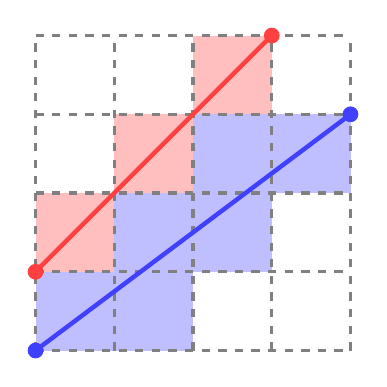
\begin{tikzpicture}
    \foreach \x/\y/\c in {
      0/0/blue, 1/0/blue, 1/1/blue, 2/1/blue, 2/2/blue, 3/2/blue,
      0/1/red, 1/2/red, 2/3/red} {
      \fill[\c!25] (\x,\y) rectangle (\x + 1, \y + 1);
    }
    \draw[gray, dashed, very thick] (0,0) grid (4,4);
    \draw[red!75, ultra thick] (0,1)--(3,4);
    \fill[red!75] (0,1) circle (0.1cm); \fill[red!75] (3,4) circle (0.1cm);
    \draw[blue!75, ultra thick] (0,0)--(4,3);
    \fill[blue!75] (0,0) circle (0.1cm); \fill[blue!75] (4,3) circle (0.1cm);
  \end{tikzpicture}
  \caption{
    An example of two lines drawn on a grid. The seven white squares
    still require a line to be drawn through them.
  }
\end{figure}

\begin{question}
  What is the minimum number of lines required to turn on all of the squares in
  and $n\times n$ grid?
\end{question}
\begin{related}
  \item What if touching the corner of a square also turns it on?
  \item What if two triangles with the same coloring but different rotations are
    counted as different?
  \item What if no two lines can be parallel?
    If no two line segments can be congruent?
  \item What if no two lines can intersect?
  \item How many fully ``on'' grids exist? How many such minimal grids? (A grid is
    minimal if removing any line results in a square turning off.)
  \item Suppose a grid is on if an even number of lines pass through it and off
    if an odd number of lines pass through it. How many such grids?
  \item How about on an $n \times m$ grid?
  \item What if this is done on a triangular grid?
  \item What if this is done on a cuboid? On a cuboid with planes passing
    through the cubes?
\end{related}
\begin{note}
  In the case where ``grid is on if an even number of lines pass through it and
  off if an odd number of lines pass through it'', there exist $2^k$
  configurations. If we further restrict to dihedral-symmetric grids, there
  are $2^j$ configurations.\\
  It appears that $k = 5n^2 - 14n + 9$, the $12$-gonal numbers. Is there a
  bijection between the basis elements and the 12-gonal numbers?
\end{note}
\end{document}
